\section{Experiments \& Measurements}
\label{sec:evaluation}

To study the design implications of the  proposed framework, a set of real-life applications was programmed and run on the tightly-coupled architecture. %Then the obtained performance of the benchmark was further compared with that achieved through pure hardware and pure software respectively. 
In addition, the soft processor was also benchmarked and compared with an existing similar RSIC-V design. Finally, resource consumption and design portability of the soft processor were evaluated to warrant the merit of the proposed framework as FPGA overlay.

\begin{table}
\begin{center}
  \caption{Parameters and configurations of the benchmarks.}
  \label{tab:tight_benchmark}

  \scriptsize
	\begin{tabular}{m{10mm}|m{16mm}|m{15mm}|m{27mm}}
    \toprule
	\bf MM  &  \bf FIR & \bf KM & \bf SE \\ 
	\hline	
	Matrix Size & \# of Input/ \# of Taps+1 & \# of Nodes/ Centroids/ Dimension & \# of Vertical Pixels/ \# of Horizontal Pixels\\
	\hline	
	100$\times$100 & 10000/50 & 5000/4/2 & (128+2)/(128+2)\\
    \bottomrule    
  \end{tabular}
\end{center}
\end{table} 

\begin{table}
\begin{center}
  \caption{The loop kernels were unrolled by the following factors before transferring to the auxiliary architecture for acceleration.}
  \label{tab:tight_unrolled}

  \scriptsize
	\begin{tabular}{m{12mm}|m{12mm}|m{11mm}|m{10mm}|m{16mm}}
    \toprule
	 & \bf MM  &  \bf FIR & \bf KM & \bf SE \\ 
	\hline	
	Full Loop & 100$\times$100$\times$ 100 & 10000$\times$ 50 & 5000$\times$ 4$\times$2 & (128+2)$\times$ (128+2)$\times$3$\times$3\\
	\hline	
	Unrolling & 1$\times$5$\times$100 & 50$\times$50 & 125$\times$4$\times$2 & 16$\times$16$\times$3$\times$3\\
    \bottomrule    
  \end{tabular}
\end{center}
\end{table} 



\subsection{Evaluation of the Tightly-coupled Architecture}
\subsubsection{Experimental Setup}
%In order to perform an accurate evaluation of the proposed architecture, the set of applications that are used to benchmark QuickDough~\cite{quickdough_fsp, quickdough} are used in this experiment. These benchmarks are essentially loop kernels which include 
Four real-life applications including matrix-matrix multiplication (MM), finite impulse response (FIR) filter, K-mean clustering algorithm (KM) and Sobel edge detector (SE) were taken as the benchmark to evaluate the tightly-coupled architecture. These applications are essentially loop kernels which are highly parallelizable and can be mapped to FPGA for performance acceleration. The parameters of the benchmark are listed in \tabref{tab:tight_benchmark}.

To understand the underlying influence of the tightly-coupled architecture (\textsc{Tightly-coupled}), the inner loop nest in each application was partially unrolled. Detailed loop unrolling configurations can be found in \tabref{tab:tight_unrolled}. The unrolled loop body was executed on a handcrafted hardware design (auxiliary architecture) for acceleration while miscellaneous loop controls and the boundary conditions that could not be covered by the accelerators were executed on the soft processor (primary architecture). The software was written in C and compiled with option \code{-O0}. 

Meanwhile, we also provided a pure hardware implementation (\textsc{HW}) and a pure software implementation (\textsc{SW}) for each of the applications for comparison. Basically, \textsc{HW} had the whole application implemented on FPGA with handcrafted hardware design. It can process not only the loop body but also the loop control as well as the boundary condition. Therefore, the execution can be done entirely on FPGA without the interventions from the soft processor. \textsc{SW} simply ignored the accelerator and had the whole application running on the proposed soft processor. The corresponding software was written in C and compiled with option \code{-O0}. 

Finally, we assumed that every piece of data was already cached in DMEM so as to eliminate the influence from the memory and maximize the impact of the soft processor architecture on the overall execution.
%in order to eliminate the influence from the memory hierarchy, we assumed that every piece of data was already cached in DMEM, which also maximizes the impact of the soft processor architecture on the overall execution.


%As mentioned in \secref{sec:implementation}, computational intensive kernels are mapped to the CGRA while the rest of the execution is handled by the soft processor according to the 90/ 10 locality rule. Therefore, in this experiments, the unrolled loop body is directed to the auxiliary architecture for acceleration while the miscellaneous loop controls and the boundary conditions are directed to the primary architecture, i.e. the soft processor to perform execution.

%However, in order to understand the underlying influence of the tightly-coupled architecture (\code{Tightly-coupled}), instead of using CGRA as the auxiliary architecture, handcrafted hardware design are used to accelerate the unrolled loop kernels. 


%In addition, in order to study the performance gain when compared with traditional software execution, C  programs for the above benchmarks are also written and they are executed on the official RISC-V Zscale core distributed by UC Berkeley~\cite{zscale}.

%Note that both \code{Tightly-coupled} and \code{HW} are running at \SI{50}{\mega\hertz} while the Zscale core is simulated at its maximum frequency \SI{500}{\mega\hertz}. The C program for the soft processor and the Zscale core is compiled with the option \code{-O0}.

\begin{figure}
    \centering
    \begin{subfigure}{0.23\textwidth}
        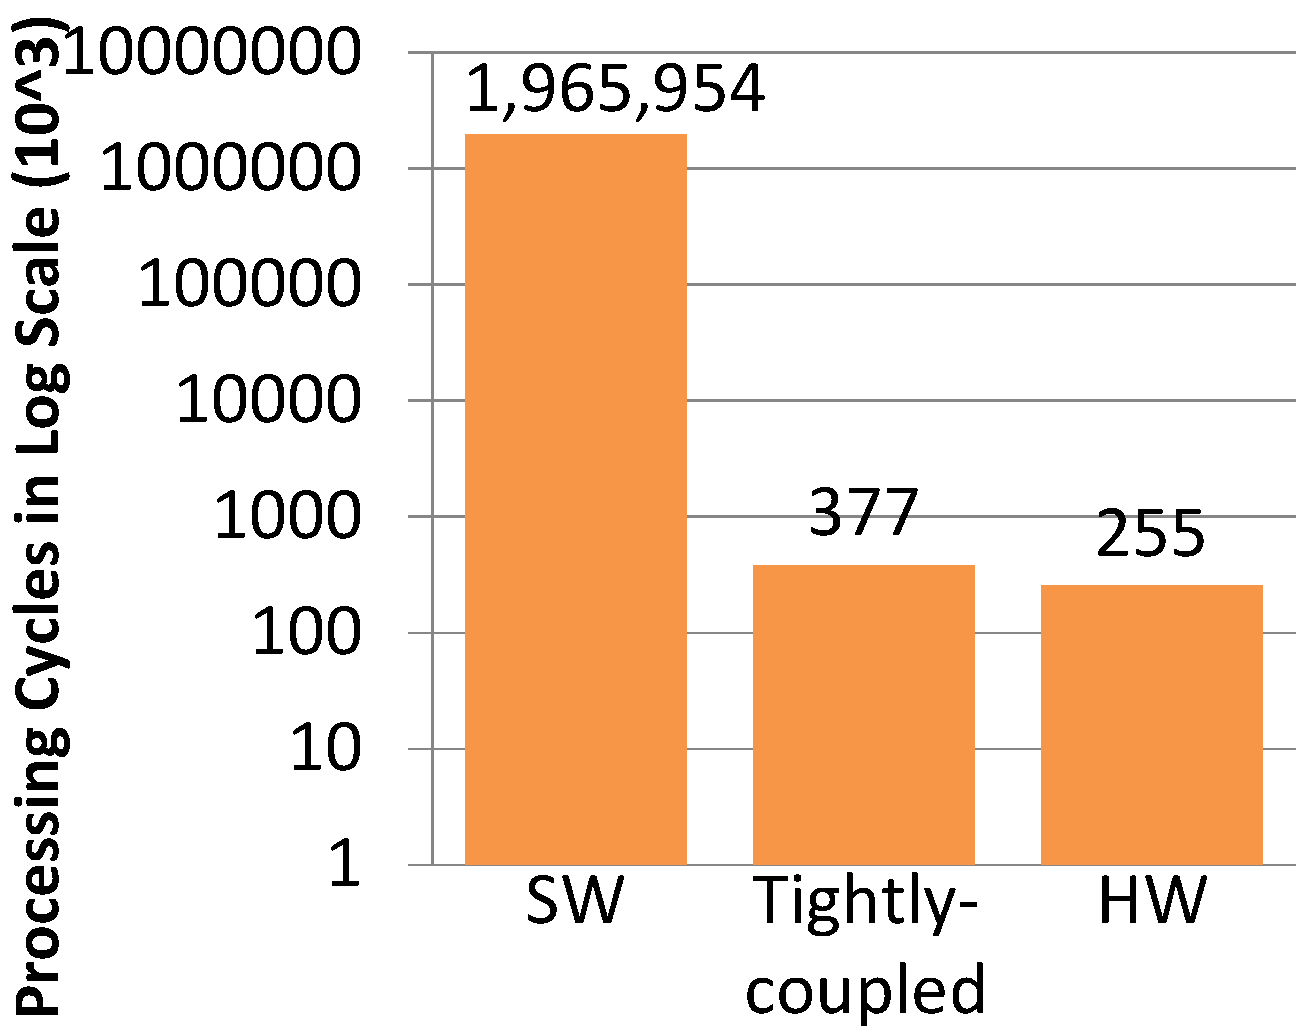
\includegraphics[width=\textwidth]{MM}
        \caption{MM}
        \label{fig:MM}
    \end{subfigure}
    ~ %add desired spacing between images, e. g. ~, \quad, \qquad, \hfill etc. 
      %(or a blank line to force the subfigure onto a new line)
    \begin{subfigure}{0.23\textwidth}
        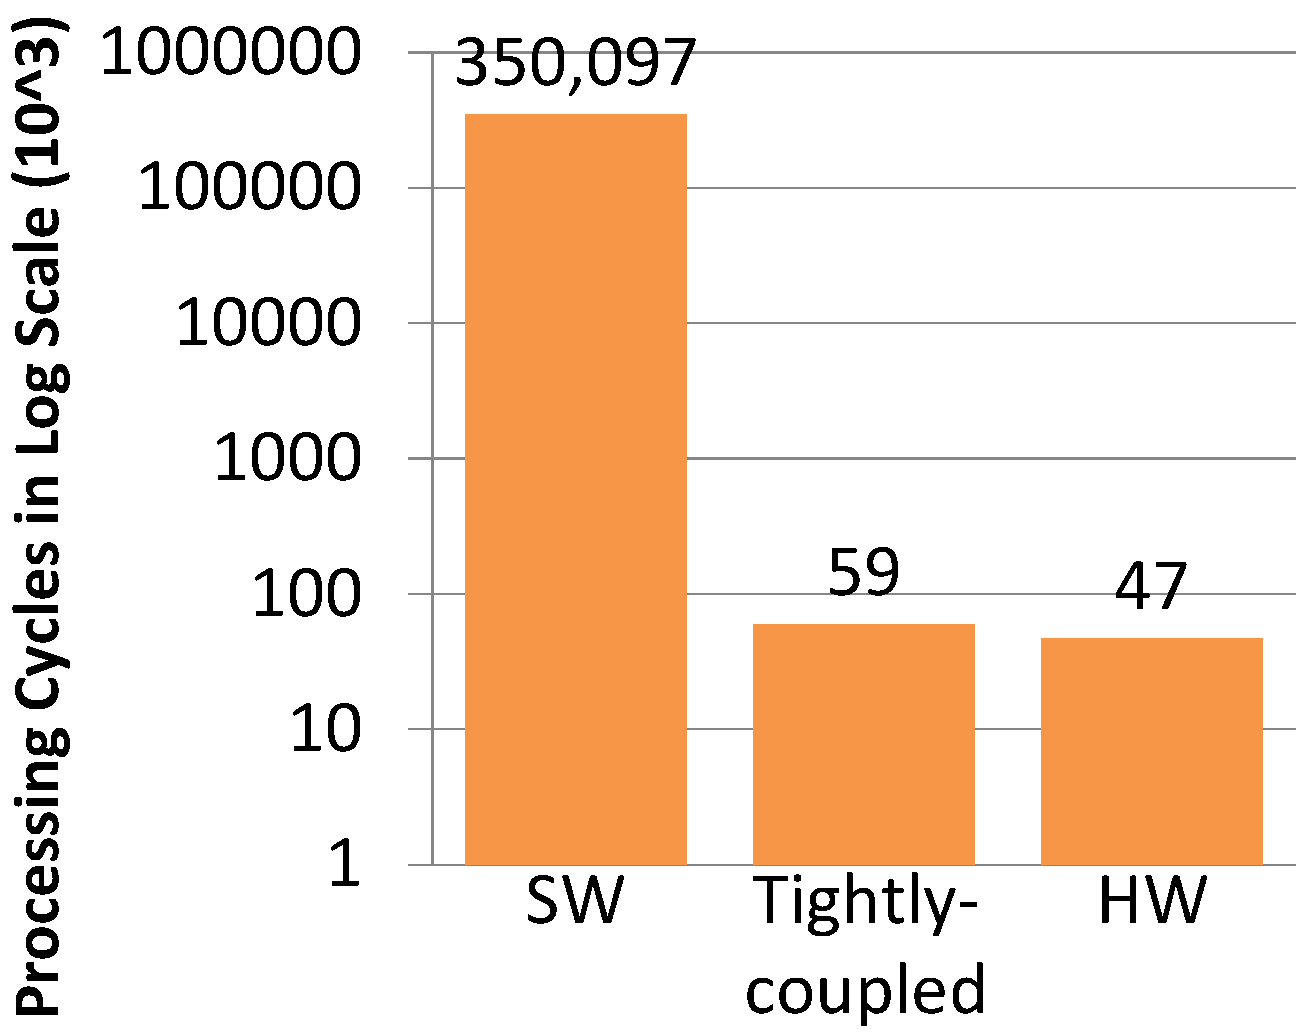
\includegraphics[width=\textwidth]{Fir}
        \caption{FIR}
        \label{fig:FIR}
    \end{subfigure}
    %\hfill
    
    ~ %add desired spacing between images, e. g. ~, \quad, \qquad, \hfill etc. 
    %(or a blank line to force the subfigure onto a new line)
    \begin{subfigure}{0.23\textwidth}
        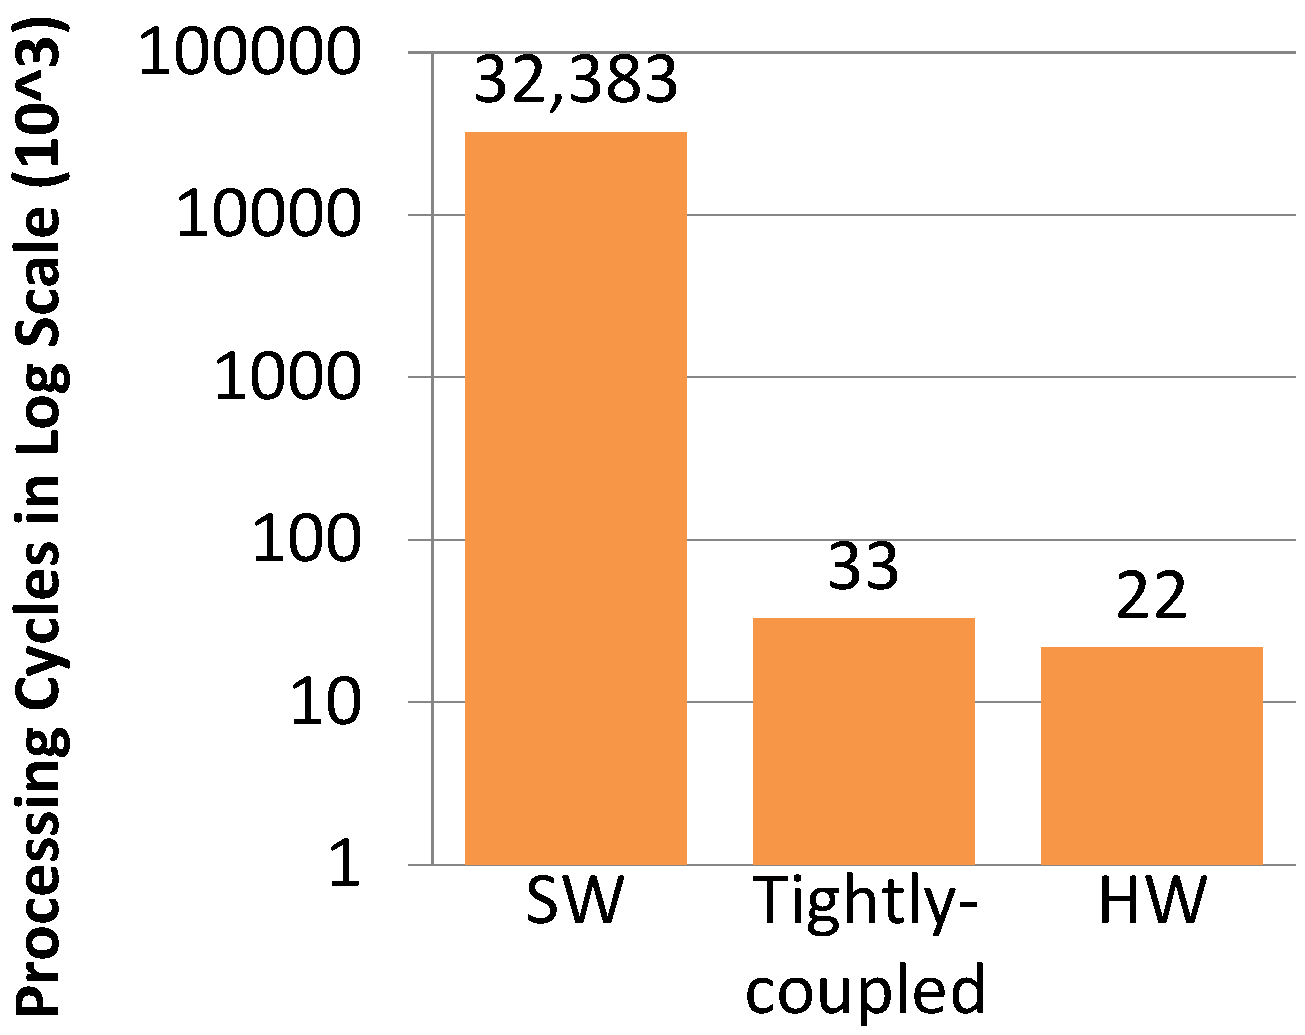
\includegraphics[width=\textwidth]{Kmean}
        \caption{KM}
        \label{fig:KM}
    \end{subfigure}
    \begin{subfigure}{0.23\textwidth}
        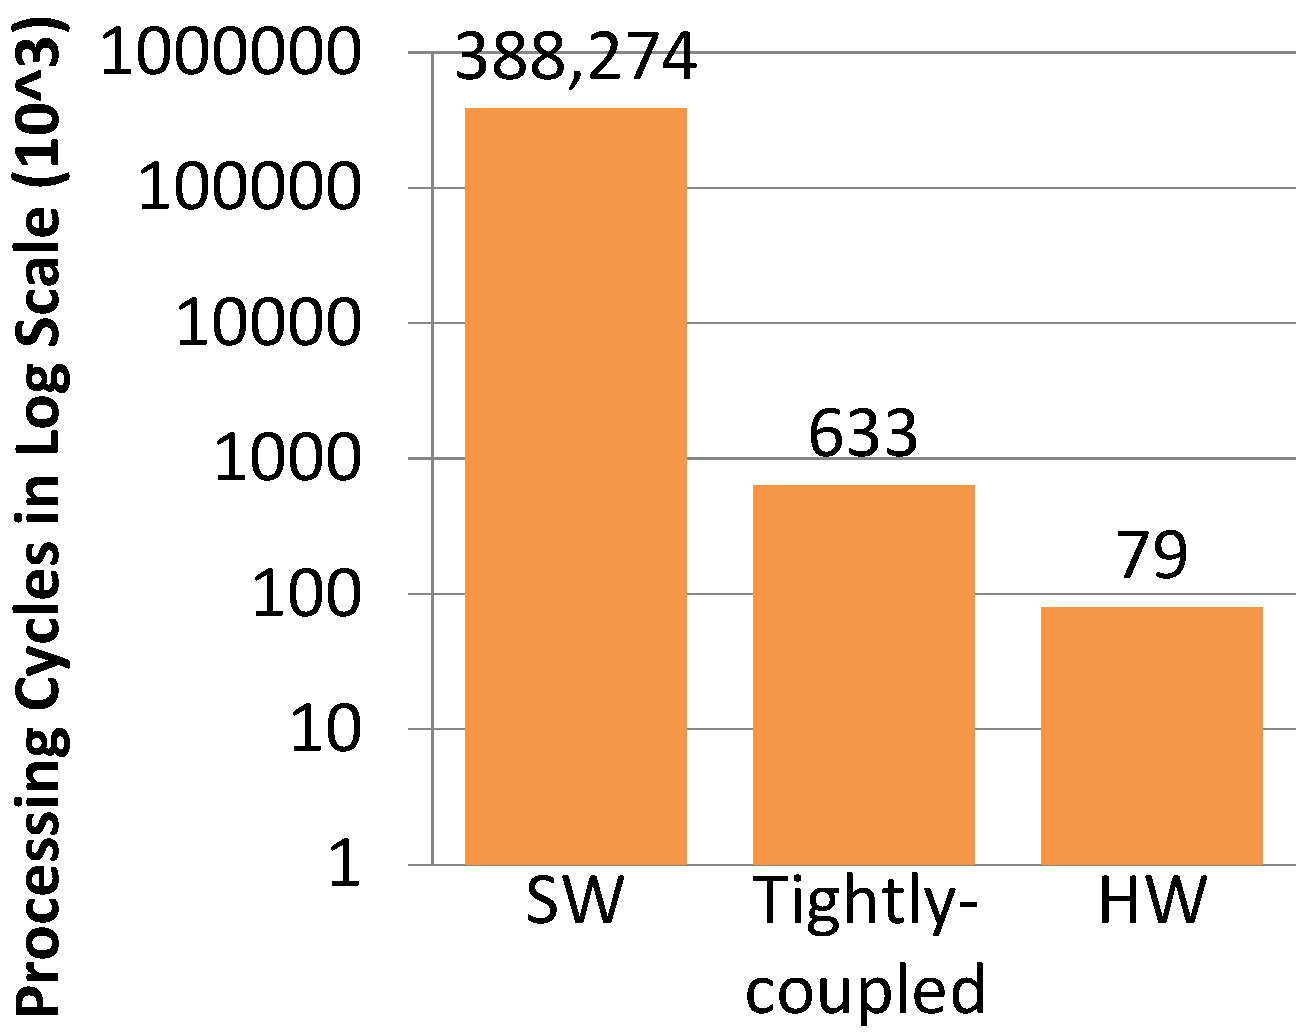
\includegraphics[width=\textwidth]{Sobel}
        \caption{SE}
        \label{fig:SE}
    \end{subfigure}
    \caption{The performance of \textsc{SW} versus \textsc{Tightly-coupled} versus \textsc{HW}. }\label{fig:tight_bench}
\end{figure}

\subsubsection{Results \& Analysis}
%Performance results of \textsc{SW} versus \textsc{Tightly-coupled} versus \textsc{HW} are displayed in \figref{fig:tight_bench} in terms of processing cycles.

As shown in \figref{fig:tight_bench}, the tightly-coupled architecture achieves similar performance when compared with \textsc{HW} in most of the benchmarks. In particular, it is found that the execution of MM, FIR and KM on \textsc{Tightly-coupled} exhibits comparable performance to that on \textsc{HW}. The main reason is that these applications only need the soft processor to handle the loop control which takes a small amount of time while they rely on the FPGA accelerators to handle the most time-consuming computing.
 
%achieve a speedup more than 60$\times$ since the soft processor is only required to handle the loop control. In addition, the handcrafted hardware designs for the unrolled loop kernels are fully-pipeline implementations that take inputs every clock cycle, therefore the overall execution latency can be extensively shortened.

In the case of SE, however, the number of processing cycles needed in \textsc{Tightly-coupled} is significantly more than that in \textsc{HW}. Such performance discrepancy is mainly caused by the following two factors. First, the boundary conditions in SE, i.e. the edge pixels, could not be covered by the auxiliary architecture for acceleration. Therefore a relatively large amount of elements (516 in this case) had to be handled by the soft processor. This would undoubtedly increase the overall execution latency. Second, SE needed the soft processor to perform a large amount of multiplication to calculate the correct memory location for a particular pixel and the entire execution latency will be lengthened consequently, especially when \code{RV32I} does not include a multiply instruction. This problem can be alleviated by extending the ISA to \code{RV32IM} and incorporating a multiplier in the soft processor design, which will be supported in the future as one of the customization parameters in the proposed framework.

%However, in the case of SE, the speedup is relatively limited and the performance gain is only about 4$\times$. The reason for such insignificant speedup is mainly because of the following two reasons. 


%\Hsection{Matrix-matrix Multiplication} The input is two $100 \times 100$ matrix (\code{M1}), (\code{M2}) and output is a $100 \times 100$ matrix (\code{M3}). 


\subsection{Evaluation of the Soft Processor}
As mentioned in \secref{sec:introduction}, though the soft processor is mostly responsible for irregular data processing and controlling over the accelerator, it is still important to have the processor to maintain sufficient efficiency while keeping the area consumption minimal. 

\subsubsection{Experimental Setup}

\begin{table}
\begin{center}
  \caption{Resource consumption and maximum frequency of the proposed soft processor versus ORCA RISC-V core.}
  \label{tab:guy_resource}
  \small
%  \begin{tabular}{p{0.8in}p{0.4in}p{0.4in}p{0.4in}p{0.4in}p{0.4in}p{0.4in}}
  \begin{tabular}{m{12mm}m{3mm}m{3mm}m{3mm}m{3mm}m{3mm}m{3mm}m{14mm}}%{lSSSSSSS}
    \toprule
%    \multirow{2}{*}{\textbf{Modules}} & \multicolumn{3}{c}{\textbf{Logic}}  &  \multicolumn{3}{c}{\textbf{Utilization}}  & FF & (\%) & BRAM &FF & LUT & BRAM\\\midrule
    \textbf{Designs} & 
    \multicolumn{2}{c}{ \begin{minipage}{0.55in}\textbf{Slice Registers}\end{minipage}}& 
    \multicolumn{2}{c}{\begin{minipage}{0.45in}\textbf{Slice LUTs}\end{minipage}}& 
    \multicolumn{2}{c}{\begin{minipage}{0.45in}\textbf{Block RAM}\end{minipage}} & 
    \begin{minipage}{0.9in}\textbf{Max. Freq.}\end{minipage}\\\midrule
      \begin{minipage}{0.5in}Proposed Soft Processor\end{minipage} & \num{334} & \SI{\sim0}{\percent} &  \num{1279} & \SI{2}{\percent} &  \num{6} & \SI{4}{\percent} & \SI{147.929}{\mega\hertz}\\\midrule
            
      \begin{minipage}{0.5in}ORCA RISC-V core\end{minipage} & \num{615} & \SI{\sim0}{\percent} &  \num{1438} & \SI{2}{\percent} &  \num{1} & \SI{\sim0}{\percent} & \SI{199.322}{\mega\hertz}\\\bottomrule
   
  \end{tabular}
  \end{center}
\end{table}


\begin{table}
\begin{center}
  \caption{Processing cycles and the execution latency of the four benchmarks on the proposed soft processor and ORCA RISC-V core.}
  \label{tab:guy_benchmark}
\renewcommand{\arraystretch}{1.5}
  \small
	\begin{tabular}{lcll}
    \toprule
	 \bf Designs & \bf Benchmarks  &  \bf \# of Cycles & \bf Latency\\ 
	 \hline	
	\multirow{4}{*}{\begin{minipage}{0.5in}Proposed Soft Processor\end{minipage}}
	 & MM & 1965954155 & \SI{13.29}{\second} \\
	 & FIR & 350096784 & \SI{2.37}{\second} \\
	 & KM & 32382531 & \SI{0.22}{\second} \\
	 & SE & 388273610 & \SI{2.62}{\second} \\
	\hline	
	\multirow{4}{*}{\begin{minipage}{0.5in}ORCA RISC-V core\end{minipage}}
	 & MM & 2868605367 & \SI{14.39}{\second} \\
	 & FIR & 503309228 & \SI{2.53}{\second} \\
	 & KM & 46286121 & \SI{0.23}{\second} \\
	 & SE & 566543126 & \SI{2.84}{\second} \\

    \bottomrule    
  \end{tabular}
\end{center}
\vspace{-2em}
\end{table} 

In order to study the efficiency of the proposed soft processor, we compared the proposed 4-stage pipeline processor with ORCA RISC-V core from VectorBlox Computing Inc.~\cite{vectorblox}. ORCA core is known as an optimized RISC-V design on FPGA that implements a 4-stage pipeline, which is most close to the proposed soft processor. Both design were implemented on Artix 7 xc7a100t-1csg324 using Xilinx ISE 14.3. Then $f_{MAX}$ as well as the resource consumption of the implementations are obtained. Meanwhile, the number of cycles that are needed to compute the benchmark are obtained from the RTL simulation.   

\subsubsection{Results \& Analysis}
\tabref{tab:guy_resource} and \tabref{tab:guy_benchmark} display the resource consumption and the performance of the proposed soft processor versus ORCA core. The percentage in \tabref{tab:guy_resource} are relative to all the available resources of the targeted FPGA device.

From these tables, we can see that the proposed soft processor typically occupies less area while at the same time providing slightly higher processing speed. The only resource that the proposed soft processor consumes more than that of ORCA core is the on-chip block RAM. This is mainly due to the existence of the IMEM and DMEM which are inferred as block RAM in the proposed processor. Such memory modules do not exist in ORCA core and hence that explains the discrepancy in block RAM consumption.


\subsection{Portability and Compatibility Considerations}
One of the major advantages of FPGA overlay is to raise the device abstraction by providing a virtual layer that is conceptually located between the user applications and the physical FPGA. Therefore, to add the soft processor to the same overlay framework with that of the accelerator, the processor must be able to support cross-vendors and cross-platforms FPGAs to ensure the device portability and compatibility.

In view of this, we have designed the processor in a generic manner such that the 4-stage pipeline design can be synthesized across various platforms ranging from Spartan-3 to Virtex-7 and Cyclone IV to V. \tabref{tab:big_resource} displays the resource consumption and the $f_{MAX}$ of the soft processor implementations on both the high-end and low-end FPGA devices. Again, the percentage in the table is relative to all the available resources on the target FPGA device.


\begin{table*}
\begin{center}
  \caption{Resource consumption and maximum frequency of the proposed soft processor on high-end and low-end FPGA devices across various generations.}
  \label{tab:big_resource}
  \renewcommand{\arraystretch}{1.3}
  \small
%  \begin{tabular}{p{0.8in}p{0.4in}p{0.4in}p{0.4in}p{0.4in}p{0.4in}p{0.4in}}
  \begin{tabular}{lSSSSSSS}
    \toprule
%    \multirow{2}{*}{\textbf{Modules}} & \multicolumn{3}{c}{\textbf{Logic}}  &  \multicolumn{3}{c}{\textbf{Utilization}}  & FF & (\%) & BRAM &FF & LUT & BRAM\\\midrule
    \textbf{Devices} & \multicolumn{2}{c}{\textbf{Slice Flip Flops}}& \multicolumn{2}{c}{\textbf{4 Input LUTs}}& \multicolumn{2}{c}{\textbf{RAMB16s}} & \textbf{Max. Freq.}\\\midrule
      Spartan3 xc3s50-5vq100 & \num{304} & \SI{19}{\percent} &  \num{1461} & \SI{95}{\percent} &  \num{2} & \SI{50}{\percent} & \SI{76.127}{\mega\hertz}\\
      
      Virtex4 xc4vfx140-11ff1517 & \num{248} & \SI{\sim0}{\percent} &  \num{1344} & \SI{1}{\percent} &  \num{4} & \SI{\sim0}{\percent} & \SI{157.351}{\mega\hertz}\\\midrule
      
      \textbf{Devices} & \multicolumn{2}{c}{\textbf{Slice Registers}}& \multicolumn{2}{c}{\textbf{Slice LUTs}}& \multicolumn{2}{c}{\textbf{Block RAM }} & \textbf{Max. Freq.}\\\midrule
      Virtex5 xc5vlx30-1ff324 & \num{280} & \SI{1}{\percent} &  \num{1081} & \SI{5}{\percent} &  \num{2} & \SI{6}{\percent} & \SI{184.735}{\mega\hertz}\\
      
      Virtex5 xc5vlx155t-3ff1738 & \num{266} & \SI{\sim0}{\percent} &  \num{1070} & \SI{1}{\percent} &  \num{2} & \SI{\sim0}{\percent} & \SI{231.913}{\mega\hertz}\\\midrule      
      

      Spartan6 xc6slx4-2tqg144 & \num{369} & \SI{7}{\percent} &  \num{1296} & \SI{61}{\percent} &  \num{10} & \SI{83}{\percent} & \SI{88.355}{\mega\hertz}\\
      
      Virtex6 xc6vhx380t-3ff1923 & \num{321} & \SI{\sim0}{\percent} &  \num{1263} & \SI{\sim0}{\percent} &  \num{6} & \SI{\sim0}{\percent} & \SI{203.198}{\mega\hertz}\\\midrule   
      
      Artix7 xc7a100t-1csg324 & \num{334} & \SI{\sim0}{\percent} &  \num{1279} & \SI{2}{\percent} &  \num{6} & \SI{4}{\percent} & \SI{147.929}{\mega\hertz}\\
      
      Virtex7 xc7vx690t-3ffg1927 & \num{318} & \SI{\sim0}{\percent} &  \num{1280} & \SI{\sim0}{\percent} &  \num{6} & \SI{\sim0}{\percent} & \SI{268.666}{\mega\hertz}\\\midrule 
  
  
    \textbf{Devices} & \multicolumn{2}{c}{\textbf{Logic Registers}}& \multicolumn{2}{c}{\textbf{Logic Elements}}& \multicolumn{2}{c}{\textbf{Memory Bits}} & \textbf{Max. Freq.}\\\midrule
      Cyclone IV EP4CE6F17C8 & \num{284} & \SI{4}{\percent} &  \num{1890} & \SI{30}{\percent} &  \SI{165888}{\kilo\bit} & \SI{60}{\percent} & \SI{68.43}{\mega\hertz}\\
      
      Cyclone IV EP4CGX75DF27C6 & \num{284} & \SI{3}{\percent} &  \num{1890} & \SI{3}{\percent} &   \SI{165888}{\kilo\bit} & \SI{4}{\percent}  & \SI{93.07}{\mega\hertz}\\\midrule    
  
  
  
      
    \textbf{Devices} & \multicolumn{2}{c}{\textbf{Logic Registers}}& \multicolumn{2}{c}{\textbf{ALM}}& \multicolumn{2}{c}{\textbf{Memory Bits}} & \textbf{Max. Freq.}\\\midrule
      Cyclone V 5CEBA2F17C8 & \num{284} & \SI{2}{\percent} &  \num{784} & \SI{8}{\percent} &  \SI{165888}{\kilo\bit} & \SI{9}{\percent} & \SI{73.5}{\mega\hertz}\\
      
      Cyclone V 5CGXFC7D6F31C6 & \num{284} & \SI{1}{\percent} &  \num{791} & \SI{1}{\percent} &   \SI{165888}{\kilo\bit} & \SI{2}{\percent}  & \SI{102.76}{\mega\hertz}\\\midrule  
   
  \end{tabular}
  \end{center}
\end{table*}
